\documentclass[a4paper,12pt]{book}

\usepackage{polski}
\usepackage[utf8]{inputenc}
\usepackage[polish]{babel}
\usepackage[unicode]{hyperref}
\usepackage{tabto}
\usepackage{graphicx}

\hypersetup{
	colorlinks=true,
	linkcolor=blue,
	filecolor=magenta,      
	urlcolor=cyan,
}
\graphicspath{ {./images/} }

\title{\Large{\textbf{Przetwarzanie Obrazów: Sprawozdanie}}}
\author{
	Damian Ubowski
	\and
	Maciej Tarach
}
\date{Warszawa, 2019}

\begin{document}
\maketitle
\tableofcontents
\chapter{Wstęp}
\section{Format obrazu}
Wybranym przez nas formatem obrazów cyfrowych jest DjVu, który jest oparty na zaawansowanej metodzie segmentacji obrazu. Tworzenie pliku DjVu polega na rozdzieleniu dowolnie skomplikowanego obrazu na odrębne warstwy, a następnie poddaniu warst odrębnym optymalizacjom i kompresjom. Format ten stosuje ładowanie progresywne, kodowanie arytmetyczne, oraz kompresję stratną dzięki czemu przy minimalnej ilości przestrzeni dyskowej można delektować się obrazami i dokumentami w wysokiej jakości. 
\subsection{Struktura formatu}
Pliki DjVu rozpoczynają się od swojej ``Magic number'' potwierdzającej rodzaj pliku i mającej wartość \textit{0x41 0x54 0x26 0x54}. Następnie czerpiąc inspirację ze struktury IFF \textbf{(Interchange File Format)} plik dzieli się na kawałki (\textit{ang. chunks}) zawierające interesujące nas cenne dane. Takie jak szerokość lub wysokość obrazu, dpi, informacje o kolorach, rozmieszczeniu pikseli, etc. Każdy kawałek składając się z ID typu, długości zawartości i samej zawartości tworzy zwarty format. Identyfikator typu określa rolę w jakiej przyjdzie służyć kawałkowi. Do dyspozycji ma ich całkiem sporo, ale uwzględniając najbardziej przydatne w naszym kontekście to ograniczymy liczbę do: 
\renewcommand{\labelitemi}{$*$}
\begin{itemize}
	\item BGjp - warstwa tylna przechowywana przy użyciu kodowania JPEG. 
	\item BFjp - warstwa przednia w formacie JPEG. 
	\item INFO - opisuje wysokość, szerokość, rozdzielczość, wersję kodera, oraz flagi wskazujące na obrót obrazu. 
\end{itemize}
\subsection{Przykładowa struktura IFF}
FORM:DJVU [14260] \newline
\tabto{5mm} INFO [10] \newline
\tabto{5mm} Sjbz [13133] \newline
\tabto{5mm} FG44 [181] \newline
\tabto{5mm} BG44 [935] \newline
\newline
Powyższa struktura przedstawia dokument składający się z jednej strony, na co wskazuje \textit{FORM:DJVU}, wraz z grafiką. Ten znacznik informuje, że mamy do czynienia z kontenerem o długości 14260 bajtów, który może zawierać inne kawałki dokumentu. Zgodnie z konwencją, po identyfikatorze typu i informacji o długości znajduje się zawartość kawałka. W tym wypadku jak i w każdym innym po \textit{FORM:DJVU} powinno znaleźć się \textit{INFO} z podstawowymi informacjami. Jeśli konwencji i wymagań specyfikacyjnych stało się zadość wtedy czas nastał na jakieś wizualne atrakcje takie jak \textit{Sjbz}, czyli masce wyboru pomiędzy kolorami z warstwy przedniej (\textit{FG44}) i tylnej (\textit{BG44}). 
\subsection{Instrukcja obsługi programu}
W celu uruchomienia kodu źródłowego będzie niezbędny: 
\begin{itemize}
	\item \href{http://djvu.sourceforge.net/}{DjVuLibre} ($\geq$ 3.5.21)
	\item \href{https://www.python.org/}{Python} ($\geq$ 2.6 lub 3.X)
	\item \href{https://cython.org/}{Cython} ($\geq$ 0.19, lub $\geq$ 0.20 dla Python 3)
	\item \href{https://wiki.freedesktop.org/www/Software/pkg-config/}{pkg-config} (POSIX)
\end{itemize}

\chapter{Operacje ujednolicania obrazów}
Ujednolicanie obrazów oznacza sprowadzenie ich do wspólnego gruntu pod względem określonego parametru. W tym wypadku będziemy ujednolicać obrazy pod względem geometrycznym (ilości kolumn i wierszy pikseli) i następnie rozdzielczościowym (wypełnienia pikselami). Sekwencyjność tych operacji jak i one same nie są w stanie spowodować spadku jakości obrazu. 
\section{Ujednolicenie obrazów szarych geometryczne}
\subsection*{Algorytm}
Algorytm geometrycznego ujednolicenia obrazów ma za zadanie sprowadzić oba obrazy do tej samej liczby pikseli w każdym wierszu i każdej kolumnie. 
\subsubsection*{Kroki algorytmu}
\begin{enumerate}
	\item Porównaj szerokości i wysokości obu obrazów i wybierz największe. 
	\item Jeśli pierwszy lub drugi obraz mają szerokość lub wysokość mniejszą od największej dostępnej to 
	wypełnij brakującą przestrzeń czarnymi pikselami. 
\end{enumerate}
\begin{figure}
	\caption{Przed uruchomieniem algorytmu (od lewej): obraz 1 (1067x1067, 300dpi), obraz 2 (2133x2133, 300dpi)}
	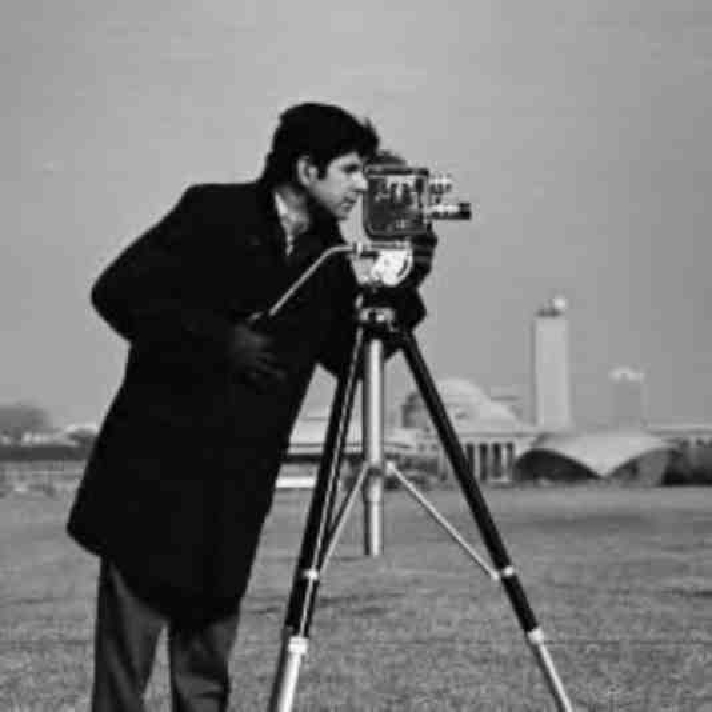
\includegraphics[width=8cm, height=8cm]{man-unmodified.jpg}
	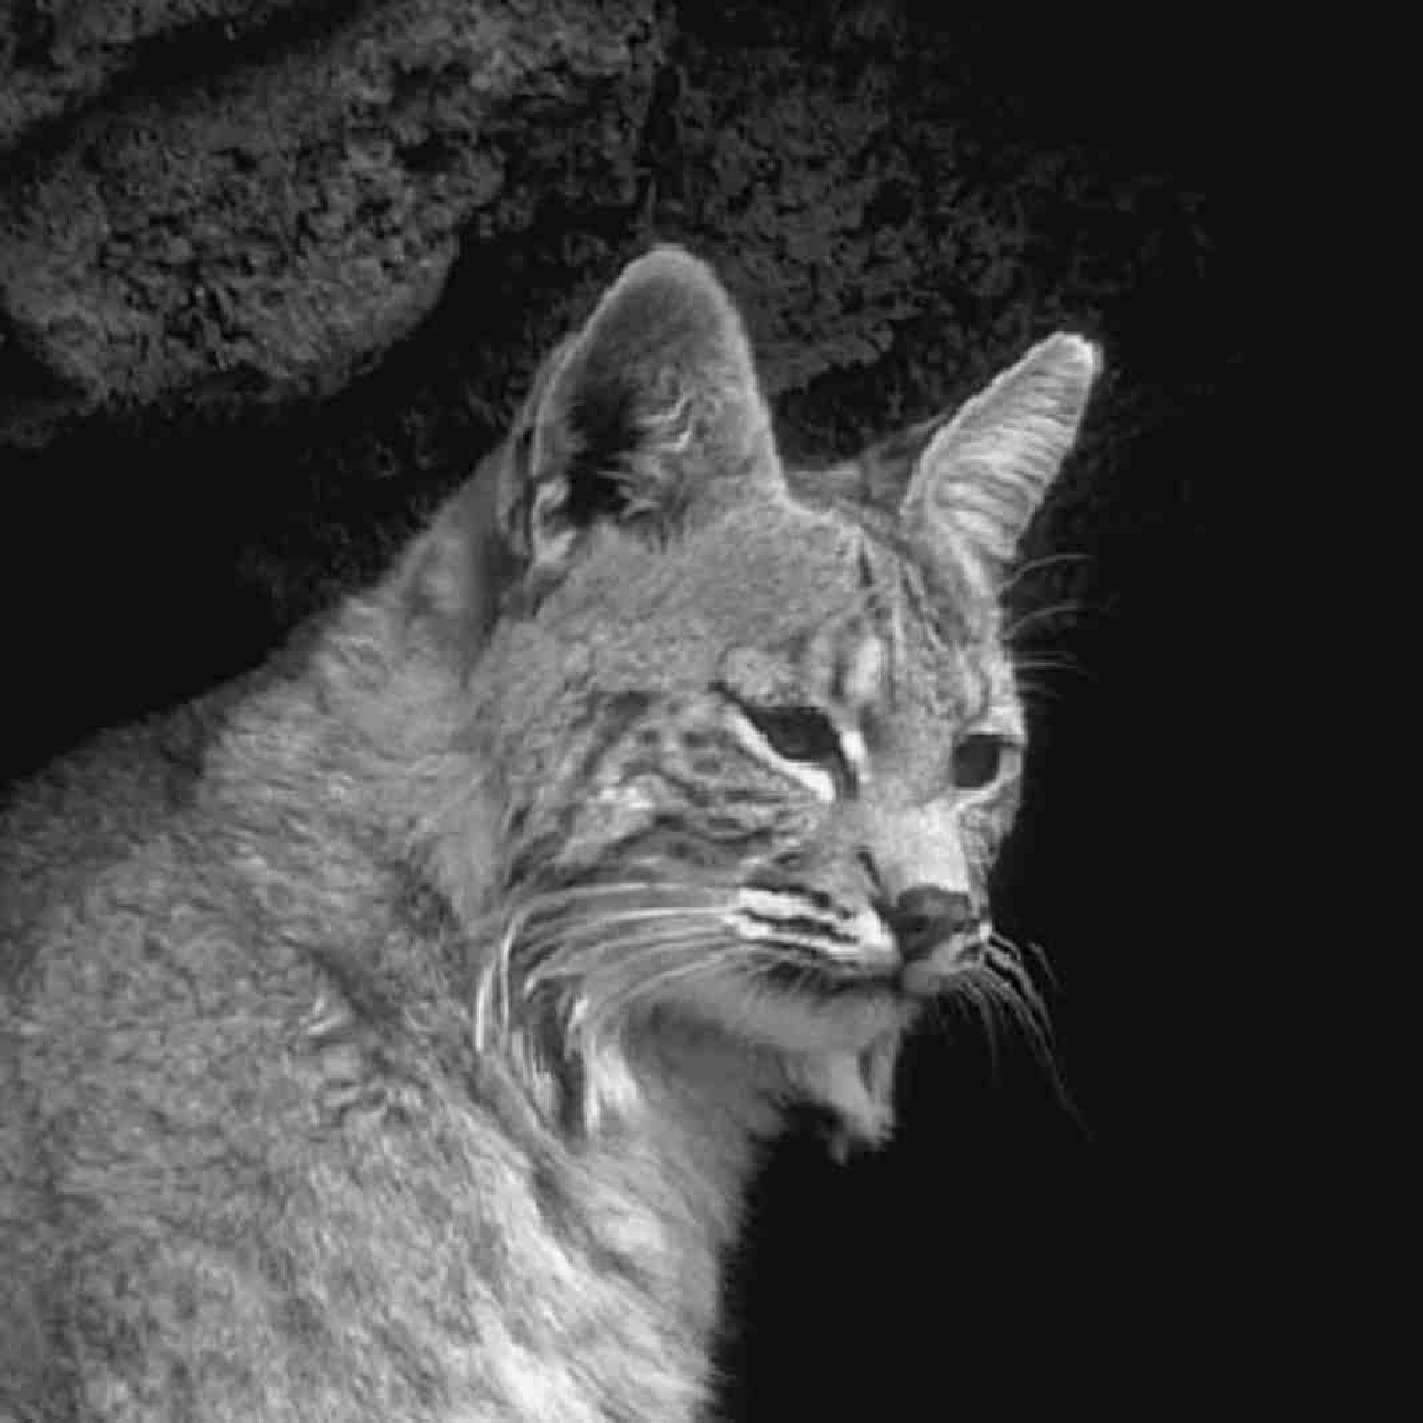
\includegraphics[width=8cm, height=8cm]{cat-unmodified.jpg}
\end{figure}
\subsection*{Kod źródłowy algorytmu}

\section{Ujednolicenie obrazów szarych rozdzielczościowe}
\section{Ujednolicenie obrazów RGB geometryczne}
\section{Ujednolicenie obrazów RGB rozdzielczościowe}

\chapter{Operacje sumowania arytmetycznego obrazów szarych}
\section{Sumowanie (określonej) stałej z obrazem}
\section{Sumowanie dwóch obrazów}
\section{Mnożenie obrazu przez zadaną liczbę}
\section{Mnożenie obrazu przez inny obraz}
\section{Mieszanie obrazów z określonym współczynnikiem}
\section{Potęgowanie obrazu (z zadaną potęgą)}
\section{Dzielenie obrazu przez (zadaną) liczbę}
\section{Dzielenie obrazu przez przez inny obraz}
\section{Pierwiastkowanie obrazu}
\section{Logarytmowanie obrazu}

\chapter{Operacje sumowania arytmetycznego obrazów barwowych}
\section{Sumowanie (określonej) stałej z obrazem}
\section{Sumowanie dwóch obrazów}
\section{Mnożenie obrazu przez zadaną liczbę}
\section{Mnożenie obrazu przez inny obraz}
\section{Mieszanie obrazów z określonym współczynnikiem}
\section{Potęgowanie obrazu (z zadaną potęgą)}
\section{Dzielenie obrazu przez (zadaną) liczbę}
\section{Dzielenie obrazu przez przez inny obraz}
\section{Pierwiastkowanie obrazu}
\section{Logarytmowanie obrazu}

\chapter{Operacje geometryczne na obrazie}
\section{Przemieszczenie obrazu o zadany wektor}
\section{Jednorodne skalowanie obrazu}
\section{Niejednorodne skalowanie obrazu}
\section{Obracanie obrazu o dowolny kąt}
\section{Symetrie względem osi układu}
\section{Symetrie względem zadanej prostej}
\section{Wycinanie fragmentów obrazu}
\section{Kopiowanie fragmentów obrazów}

\chapter{Operacje na histogramie obrazu szarego}
\section{Obliczanie histogramu}
\section{Przemieszczanie histogramu}
\section{Rozciąganie histogramu}
\section{Progowanie lokalne}
\section{Progowanie globalne}

\chapter{Operacje na histogramie obrazu barwowego}
\section{Obliczanie histogramu}
\section{Przemieszczanie histogramu}
\section{Rozciąganie histogramu}
\section{Progowanie 1-progowe lokalne}
\section{Progowanie wielo-progowe lokalne}
\section{Progowanie 1-progowe globalne}
\section{Progowanie wielo-progowe globalne}

\chapter{Operacje morfologiczne na obrazach binarnych}
\section{Okrawanie (erozja)}
\section{Nakładanie (dylatacja)}
\section{Otwarcie}
\section{Zamknięcie}

\chapter{Operacje morfologiczne na obrazach szarych}
\section{Okrawanie (erozja)}
\section{Nakładanie (dylatacja)}
\section{Otwarcie}
\section{Zamknięcie}

\chapter{Filtrowanie liniowe i nieliniowe}
\section{Filtr dolnoprzepustowy uśredniający}
\section{Filtr dolnoprzepustowy Gaussowski}
\section{Operator Roberts’a}
\section{Operator Prewitt’a}
\section{Operator Sobel’a}
\section{Filtr kompasowy}
\section{Gradient wektora kierunkowego}
\section{Filtr medianowy}
\section{Filtr maksymalny}
\section{Filtr minimalny}
\section{Filtr płaskorzeźbowy}

\end{document}